\documentclass[11pt,compress,t,notes=noshow, aspectratio=169, xcolor=table]{beamer}

\usepackage[nospeakermargin]{../../style/lmu-lecture-2}
% Defines macros and environments
\input{../../style/common.tex}
\usepackage{pax}
\setbeamertemplate{frametitle}{\expandafter\uppercase\expandafter\insertframetitle}
%\useoutertheme{metropolis}
% remove section slides
\AtBeginSection[]
{
	\begin{frame}<beamer>
		\frametitle{Advanced Machine Learning}
		\tableofcontents[currentsection]
	\end{frame}
}
% includepdf slides, pagecommad will set counter for framenumber
\usepackage{pdfpages}
\includepdfset{trim=0mm 0mm 0mm 0mm, pagecommand={\global\setcounter{framenumber}{\value{page}}}}
% trim=0mm 6mm 0mm 0mm, offset=0 15,
% add footer:
\usepackage{framed, color}
\usepackage{xcolor}
%\iffalse
\setbeamertemplate{footline}[text line]{%
	\noindent\hspace*{\dimexpr-\oddsidemargin-1in\relax}%
	\colorbox{white}{
		\makebox[\dimexpr\paperwidth-2\fboxsep\relax]{
			\color{black}
			\begin{minipage}[c][2ex][c]{0.5\linewidth}
				\secname
			\end{minipage}
			\hfill\begin{minipage}[c][2ex][c]{0.5\linewidth}
				\flushright
				\insertframenumber{}~/~\inserttotalframenumber~~
			\end{minipage}
	}}%
	\hspace*{-\paperwidth}
}
%\fi
\title{Applied Machine Learning}
% \author{LMU}
%\institute{\href{https://compstat-lmu.github.io/lecture_iml/}{compstat-lmu.github.io/lecture\_iml}}
\date{}

\begin{document}

\newcommand{\titlefigure}{figure/empty}
\newcommand{\learninggoals}{
\item Imputation}

\lecturechapter{Imputation}
\lecture{Applied Machine Learning}

\section{Imputation}
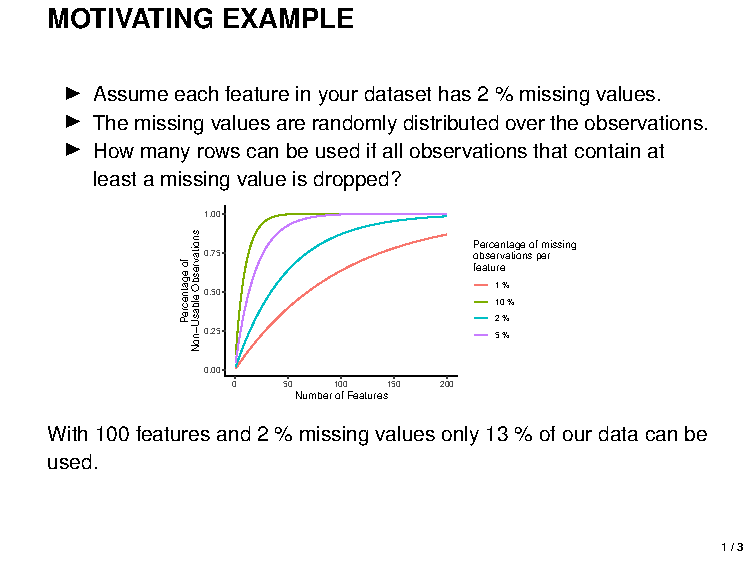
\includepdf[pages={1-last}]{pdf_chapters/slides_01_imputation_intro.pdf}
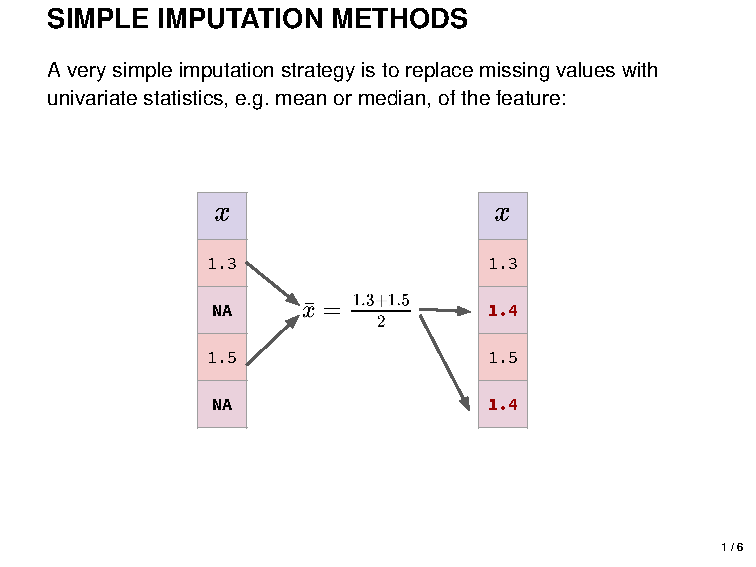
\includepdf[pages={1-last}]{pdf_chapters/slides_02_imputation_simple.pdf}
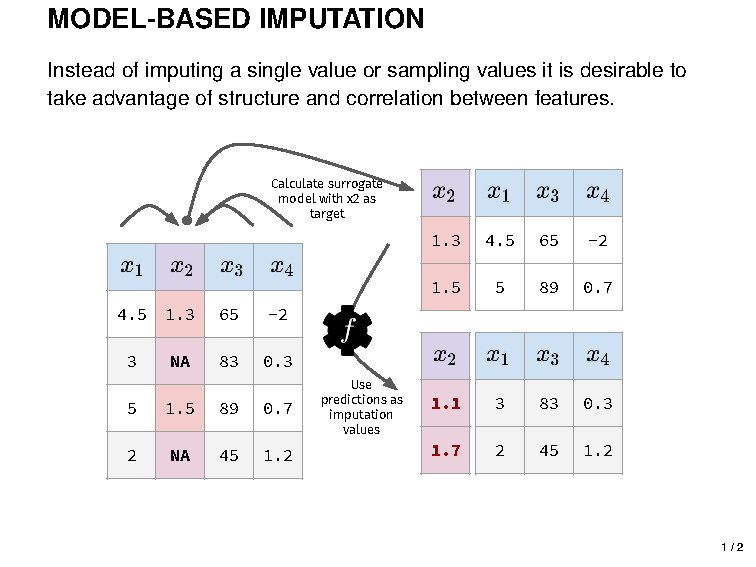
\includepdf[pages={1-last}]{pdf_chapters/slides_03_imputation_models.pdf}
\endlecture
\end{document}
